\chapter{Neural Networks}
\begin{quotation}
\noindent ``\emph{To a man with a hammer, everything looks like a nail.}''
\begin{flushright}\textbf{Mark Twain}\end{flushright}
\end{quotation}

\vspace*{0.5cm}

Throughout this paper, we will use the very powerful tool that a neural network
is for several different purposes. One could describe a neural network in 
three words: general function approximators. We can describe their input
and the output desired from that input -- inbetween stands a very large amount of
nonlinear computations of which coefficients and parameters can be tuned to
make the network's output closer to what we want in a process called training, 
or learning. The name "neural network"
barely hides the analogy with how human neurons function -- and although there
are similarities to how humans learn, the analogy stays very much a conceptual
analogy, and artificial neural networks stay orders of magnitude less complex
than the billions and billions of interconnected neurons humans have developed. 

\section{Feedforward neural networks}
A neural network is a collection of interconnected \textit{neurons}. The
reason why neurons bear this name is because of their similarity to 
human neurons. Each neuron is a computational unit which takes input
from several other neurons (via synapses if one wishes to push the analogy further)
and transforms this input into an output value, which will then be carried on
to the following neurons.\\

The simplest and most widely used networks are feedforward neural networks. In
this setting, neurons are arranged into ordered layers of which the first one is
called the input layer, the last one is called the output layer and
intermediate layers are called hidden layers
(see Figure~\ref{fig:neural_network}). Having neurons arranged in layers
means that each neuron in a layer takes input from each of the neurons
in the previous layer and outputs to each of the neurons in the next layer.\\

The input vector, also called the feature vector \index{feature vector},
is composed of \textbf{features} (measurements, properties,...). Say
for example that we wanted to build a neural network that classifies cats and
dogs; we could measure attributes such as the height of the animal, the length
of its hair, its general loyalty to its owners and the number of hours it 
spends sleeping per day and try to build a neural network that classifies
them based on these features.\\

For the output layer, we would have a two-neuron layer: one which corresponds
to "cat" and the other one to "dog". Once we have trained the network
(see Section~\ref{nn:training}), the neuron that has the highest value
after distilling the input values through the network would specify the
kind of animal the neural network thinks the measurements best fit to.\\

\begin{figure}[]
	\centering
	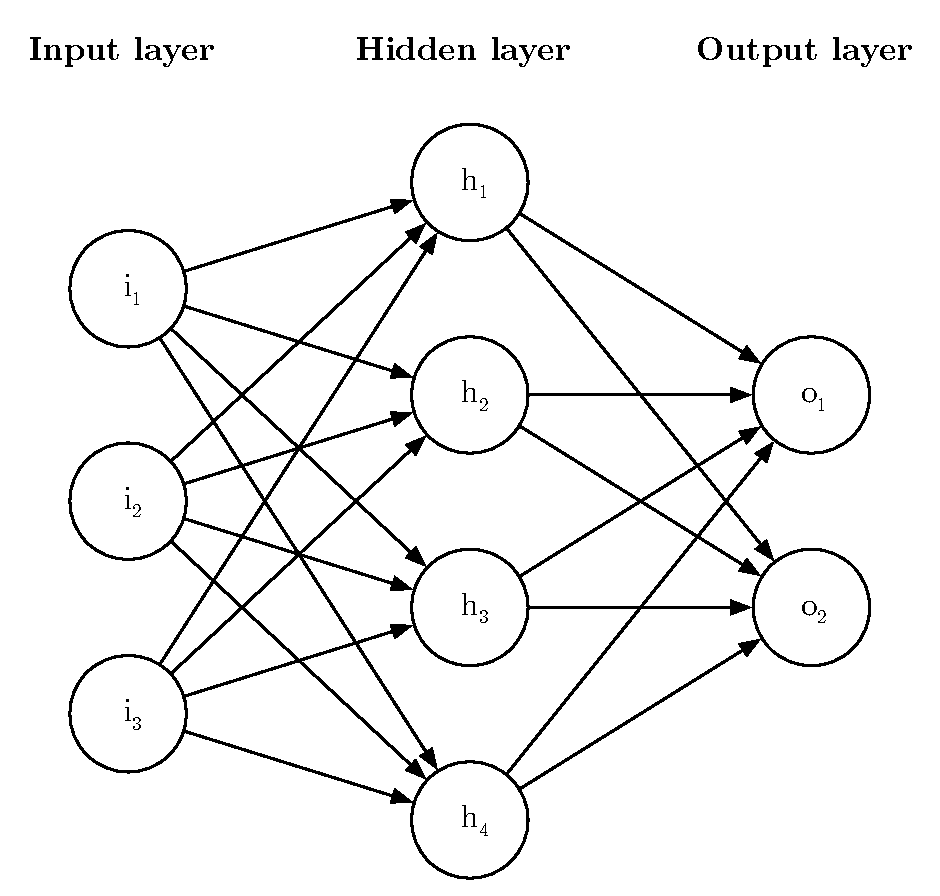
\includegraphics[width=0.6\linewidth]{fig/neural_network.eps}
	\caption{A neural network with one input layer composed of three neurons,
	one hidden layer of 4 neurons, and one output layer with 2 neurons.}
	\label{fig:neural_network}
\end{figure}


In a feedforward neural network, each neuron is connected to every neuron in 
the next layer.  To obtain an output from a given input,
the information will be passed from layer to layer in the following way: 
each neuron computes a weighted sum of the outputs of all neurons in the
previous layer then squashes this weighted sum in an activation function.
\index{activation function} 
Hence, the neuron $h_1$ in the network of Figure~\ref{fig:neural_network}
outputs:
$$ f(w_1i_1 + w_2i_2 + w_3i_3 + b) $$
where $w_1, w_2, w_3$ are the weights \index{weights} corresponding to the
connections between $i_1, i_2, i_3$ and $h_1$; and $b$ is a bias term. 
These weights are the learnable parameters of any neural network and will be 
tuned during training to improve the accuracy of the network. 
The activation function $f(\cdot)$ can be chosen arbitrarily, as long as it 
is differentiable \footnote{This is mostly true, although some activation
functions that have recently been made popular because of their good
performance such as Rectified Linear Units (ReLUs) \cite{relus} are not 
differentiable on all of their domain.}
(so that backpropagation can work, see \ref{nn:training})
but it is the same for all the neurons in the same layer. Some options are
the sigmoid function, the hyperbolic tangent function and sometimes a simple
linear function.\\

The reader might have noticed that using matrices is an efficient way of writing
and executing computations within a neural network. Indeed, one could write
the computation between the input layer and the first hidden layer as: 

$$ h = f_h(iW_{ih} + b_h) $$

\noindent where : 
\begin{itemize}
	\item $h$ is a $1\times n$ vector containing the values of the neurons 
		in the hidden layer
	\item $i$ is a $1\times m$ vector containing the values of the neurons
		in the input layer
	\item $W_{ih}$ is a $m\times n$ matrix containing the weights between
		the input and hidden layer
	\item $b_h$ is the $1\times n$ bias vector 
	\item $f_h$ is the activation function choosen for the hidden layer
\end{itemize}

Similarly, the computation between the hidden layer and the output layer
can be written as:
$$ o = f_o(hW_{ho} + b_o) $$
Hence the full transformation between the input and the output is:
$$ o = f_o\left(f_h(iW_{ih} + b_h)W_{ho} + b_o\right) $$

The example of Figure~\ref{fig:neural_network} is an extremely simple example.
Often, neural networks will be \textbf{wider} (meaning that there are more
neurons per layer) and \textbf{deeper} (meaning that there will be more layers).
This can lead to issues and challenges when training them. The main issue
related to deep neural networks is the vanishing gradient problem, exposed
by Hochreiter \cite{vanishing_gradient}. More generally, adding more 
neurons (or units) increases the possibility of \textbf{overfitting} (see
Section~\ref{sec:regularisation}).

\subsection{Training}
\label{nn:training}
Every neural network is initialised randomly at first, meaning that we will
attribute a random value (that is sampled from a user-defined distribution)
to each weight in the network.\\

If we want to train a network to differentiate a cat from a dog based on a
given set of measurements, we will have to expose it to a large number of examples
of measurements and their associated ground truths \index{ground truth}
(whether the measurements actually correspond to a cat or a dog). This large
number of examples is called the \textbf{training set} $\mathcal{D}$. 
\index{training set} Training is
then performed by alternating feedforward passes (distilling the input through
the network and obtaining the network output) and backpropagation: modifiying 
the weights of the connections between neurons (that will in turn modify 
the network output) until the network output matches the ground truth with 
a good enough accuracy.\\

The forward pass has been explained previously, but the backwards pass, also
called \textbf{backpropagation}, is slightly more complicated.\\

\subsubsection{Loss function}
The first thing we need to improve our network is a number which measures
how far the network output is from the ground truth.
This is exactly what a \textbf{loss function} \index{loss function} does: 
it describes numerically the error between the target and the network output.
One example of a loss function is the mean square error (MSE) \index{MSE} which
is very useful in regression problems:
$$ \mathcal{L}_{\text{MSE}} = \sum\limits_{(x, t) \in \mathcal{D}}\frac{(f(x)-t)^2}{|\mathcal{D}|}$$
where $x$ is a feature vector, $t$ is its corresponding ground truth and $f$
is our model. In
many cases, $f(x)$ and $t$ are vectors, so we may sum or average the loss computed
over components.\\

For classification problems, like the cats and dogs example, one typically uses
a cross-entropy loss which is defined as the following for one sample:
$$-\sum\limits_c t_c\log(f(x)_c)$$
where $c$ is the class index, hence the loss computed over the whole dataset being:
$$\mathcal{L}_{\text{CE}} = \sum\limits_{(x, t) \in \mathcal{D}}
\frac{-\sum\limits_c t_c\log(f(x)_c)}{|\mathcal{D}|}$$
In our cats and dogs example, let us consider that the ground truth for
"cat" corresponds to the output vector $[1, 0]$ and the ground truth for "dog"
corresponds to the output vector $[0, 1]$. If the network predicts $[0.3, 0.7]$
when it is given measurements of a cat, the loss function will equate to :
$$ \mathcal{L} = -(1\log(0.3) + 0\log(0.7)) = -0.47$$
whereas if it had predicted $[0.9, 0.1]$, the loss would have equated to:
$$ \mathcal{L} = -(1\log(0.9) + 0\log(0.1)) = -0.95$$

The experienced reader might already have concluded that since we want to
minimise the loss function, we are confronted with an optimisation problem.

\subsubsection{Backpropagation}
\index{backpropagation}
We will only summarise backpropagation in this section as explaining it in
full is out of the scope of this paper.
\todo{remove}
The problem at hand is indeed an optimisation problem with the following
parameters:
\begin{itemize}
	\item the objective function, which we want to minimise, is the loss 
		function
	\item the parameters are all the weights of the neural network
\end{itemize}
How can we link the parameters to the objective function? A key requirement
for activation functions and the loss function is that they have to be
\textbf{differentiable}. When this is the case, we can compute the gradient
of the loss function (in other words, the gradient of the error) and 
backpropagate it through the network by using the
chain rule of derivation. The derivative of the loss function can be written
in terms of its partial derivatives with respect to each of the weights
in the network:
$$\nabla\mathcal{L} = \left(
  \frac{\delta\mathcal{L}}{\delta w_1}, 
  \frac{\delta\mathcal{L}}{\delta w_2}, 
  \frac{\delta\mathcal{L}}{\delta w_3}, ...,
  \frac{\delta\mathcal{L}}{\delta w_k}\right) 
$$
Each weight will then be modified by adding a small increment in the direction 
of the gradient:
$$ \Delta w_i = - \alpha \frac{\delta\mathcal{L}}{\delta w_i}$$
where $\alpha$ is the learning rate, a hyperparameter chosen by the designer
of the network that defines the size of the steps to make in the direction
of a smaller error. A high learning rate may accelerate training but could
reduce the chance of finding a global optimum. Reducing the learning rate,
on the other hand, could make the training slower but at the same time 
increase the probability of finding a global optimum.\\

Let us derive the gradient of a weight which connects a neuron in the 
last hidden layer to a neuron in the output layer in the case
where we have a MSE loss:
$$ \Delta w_{oh} = -\alpha\frac{\delta\mathcal{L}}{\delta w_{oh}}$$
which can be expanded using the chain rule:
\begin{equation}
\Delta w_{oh} = -\alpha
\frac{\delta\mathcal{L}}{\delta a_o}
\frac{\delta a_o}{\delta net_o}
\frac{\delta net_o}{\delta w_{oh}}
	\label{eq:chainrule}
\end{equation}
where $net_o$ is the input of neuron $o$ and $a_o$ is the activation value
of neuron $o$.\\

Let us analyse each partial derivative of equation~\ref{eq:chainrule}.
The derivative of the error with respect to the activation is :
$$ \frac{\delta\mathcal{L}}{\delta a_o} = 
\frac{\delta(\frac{1}{2}(t_o-a_o)^2)}{\delta a_o} = -(t_o-a_o)$$
Notice that we injected a $\frac{1}{2}$ factor to the error to simplify 
computations.\\

The derivative of the activation with respect to the input of the neuron is:
$$ \frac{\delta a_o}{\delta net_o} $$
It is simply the derivative of the activation function chosen for
the output layer. Since this derivative will vary depending on the choice
of activation function, we will simply denote is as $f_o'$.\\


The derivative of the neuron input with respect to the weight is
$$ \frac{\delta net_o}{\delta w_{oh}} = \frac{\delta (w_{oh}a_h)}{\delta w_{oh}}
 = a_h$$

Hence we will update a weight between the last hidden layer and the output
layer with:
$$ \Delta w_{oh} = \alpha (t_o-a_o)f_o'(net_o)a_h$$

For weights that connect the penultimate hidden layer to the last layer (in
our case, the input layer to the hidden layer), the error is slightly more 
complicated as it depends on the error of all $k$ neurons in the hidden layer,
and not just of one output neuron. The gradient of such a weight can be
written as:
\begin{equation}
\Delta w_{hi} = -\alpha
	\sum\limits_k \left(
	\frac{\delta\mathcal{L}}{\delta a_k}
	\frac{\delta a_k}{\delta net_k}
	\frac{\delta net_k}{\delta a_h}
	\right)
\frac{\delta a_h}{\delta net_h}
\frac{\delta net_h}{\delta w_{hi}}
	\label{eq:chainrule_further}
\end{equation}
A similar reasoning can be used to unfold equation \ref{eq:chainrule_further}.

Backpropagation uses the fact that activation functions are differentiable to
perform gradient descent. Indeed, the error signal is a surface in a space
of which the dimensionality is equal to the number of parameters in the
network. Gradient descent aims to find the global minimum of this error
surface.\\


\subsubsection{Summary}
To train a neural network, its weights have to be randomly initialised first,
then we show it many examples of the training set, containing measurements and
ground truths. For each of these examples, or samples:
\begin{enumerate}
	\item the feedforward pass computes the network output from the sample
		input data
	\item the network output is compared with the sample output and the
		error signal given by a loss function
		is backpropagated through the network, updating
		all the weights
\end{enumerate}

\subsection{Testing, overfitting and regularisation}
\label{sec:regularisation}
So far, we only discussed training neural networks, but testing and
evaluating their performance is just as important. Indeed, as hinted at
previously, there is a chance that neural networks \textbf{overfit}. This
means that the network will learn a function which fits the training data
very well, but that doesn't \textbf{generalise} to new data. We use
another dataset, the \textbf{validation} set, which contains pairs of feature
vectors and their associated ground truths that have never been seen by the
model during training. If the performance of the network is much lower on
the validation set than on the training set, we know that it has overfit
the training data. We use the validation set to test different 
values of hyperparameters (number of layers, size of layers, learning rate,...),
and we choose the combination of hyperparameters and overfitting avoidance
techniques that minimise the error on the validation set.\\

\todo{figure}

There are several ways of avoiding overfitting, of which some are:
\begin{itemize}
	\item \textbf{dropout} \cite{dropout} which "disables" neurons in the 
		network with a certain probability during training. This allows
		for a large combination of thinner sub-networks to learn
		separately from other sub-networks.
	\item adding more data, or augmenting the existing data by transforming
		it can also increase generalisation performance as the network
		won't "remember" a given set of examples as opposed to truly
		trying to understand the concepts we want it to learn
	\item \textbf{early stopping} is a method that checks the error
		on the validation set during training, and that stops training
		whenever the error on the validation set starts increasing.
		The increase of validation error will usually mean that the
		network has started overfitting the training data.
\end{itemize}

Finally, when we have minimised the error on the validation, we use 
a \textbf{test set}. This set contains new pairs of feature vectors and their
targets that are neither in the training set nor the validation set. Using
a test set helps avoiding overfitting the \textit{hyperparameters} of the model.
Indeed, finding the hyperparameters that minimise the error on the validation
set is a sort of overfitting; and running the model on completely unseen
data from the test set gives a true estimation of the generalisation performance
of our model. Once this estimation has been made, we cannot tune the model
any further (or we would have to use a different test set).

\section{Recurrent neural networks}
There is one limitation to feedforward neural networks which can be particulary
critical for some applications. Very often, having an output mapped to a 
single input is not enough. For example, in problems where samples are organised
in a timeline and dependent on each other, only seeing one input at a time
does not provide enough information. If one wants to predict the weather
temperature in the next hour, it would be useful to know more than only the
last ground truth value to identify a potential trend. One 
could input a fixed-size window of the previous time steps to the network,
but this approach limits the scope of available "memory" and could dramatically
increase the complexity of the model.\\

One solution to this problem is the use of recurrent neural networks.
A feedback loop such as the one shown in Figure~\ref{fig:rnn}a, also called
a recurrent connection, means that the layer at the receiving end of the
recurrent connection will receive as input not only the value of the previous
layer at time $t$, but also the value of the layer at the giving end of the 
recurrent connection at time $t-1$. This allows information to \textit{live}
throughout time steps.\\

A recurrent connection, however, poses evident issues for the backpropagation
algorithm since the depth of the neural network can become theoretically
infinite.  A common way of training and visualising recurrent neural networks 
is to unroll them for a given, finite amount of time steps (see 
Figure~\ref{fig:rnn}b).  The error signal can then be computed
for the output value at each time step, and backpropagated through all the
previous input values that affected its computing.\\
\begin{figure}[]
	\centering
	\subfloat[][A recurrent connection]{\qquad
		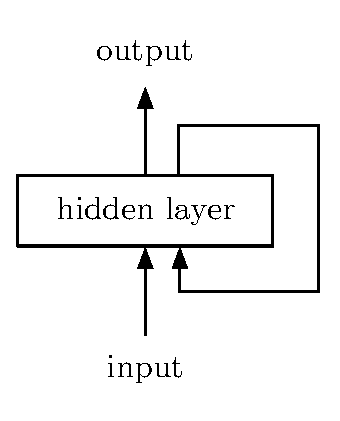
\includegraphics[width=0.1515\linewidth]{fig/recurrent_neural_network.eps}\qquad}
	\qquad
	\subfloat[][An unrolled recurrent neural network]{
		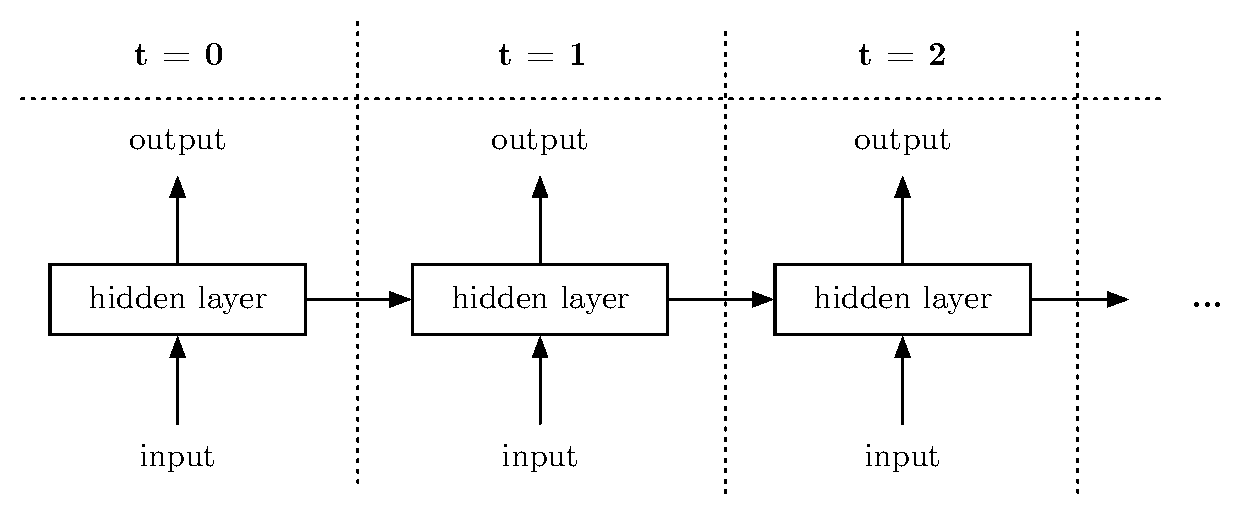
\includegraphics[width=0.6\linewidth]{fig/recurrent_neural_network_unrolled.eps}}
	\caption{Recurrent neural networks}
	\label{fig:rnn}
\end{figure}


Backpropagation through time \cite{bptt} works conceptually in the same way
as normal backpropagation. For a sequence of 3 steps such as the one shown
on Figure~\ref{fig:bptt}, we consider that the network has 3 layers. 
One key difference with standard backpropagation is that the weights
between each layer are actually the same since we only unrolled the network.
The equations of backpropagation have to be slightly adapted to perform
gradient descent on the recurrent weights. The partial derivative of the
loss function at $t=3$ with respect to the recurrent weights is:
\begin{equation}
	\frac{\delta\mathcal{L}_3}{\delta W_{hh}} = 
\frac{\delta\mathcal{L}_3}{\delta a_o}
\frac{\delta a_o}{\delta net_o}
\frac{\delta net_o}{\delta W_{hh}}
	\label{eq:chainrule_bptt}
\end{equation}
but this time, $net_o$ depends on $net_{h_3}$ which in turn depends on $W_{hh}$, so
when we take its derivative with respect to $W_{hh}$, we cannot take it as
a constant. The equation has to be unfolded like this:
\begin{equation}
	\frac{\delta\mathcal{L}_3}{\delta W_{hh}} = 
	\sum\limits_{k=0}^2
\frac{\delta\mathcal{L}_3}{\delta a_o}
\frac{\delta a_o}{\delta net_o}
\frac{\delta net_o}{\delta net_{h_k}}
	\frac{\delta net_{h_k}}{\delta W_{hh}}
	\label{eq:chainrule_bptt}
\end{equation}

Unrolled recurrent neural networks are just deep neural networks, and the
more they are unrolled, the deeper they get, so they also suffer from
the vanishing or exploding gradients problem \cite{vanishing_gradient_rnn}.
\todo{maybe explain}

\begin{figure}
	\centering
	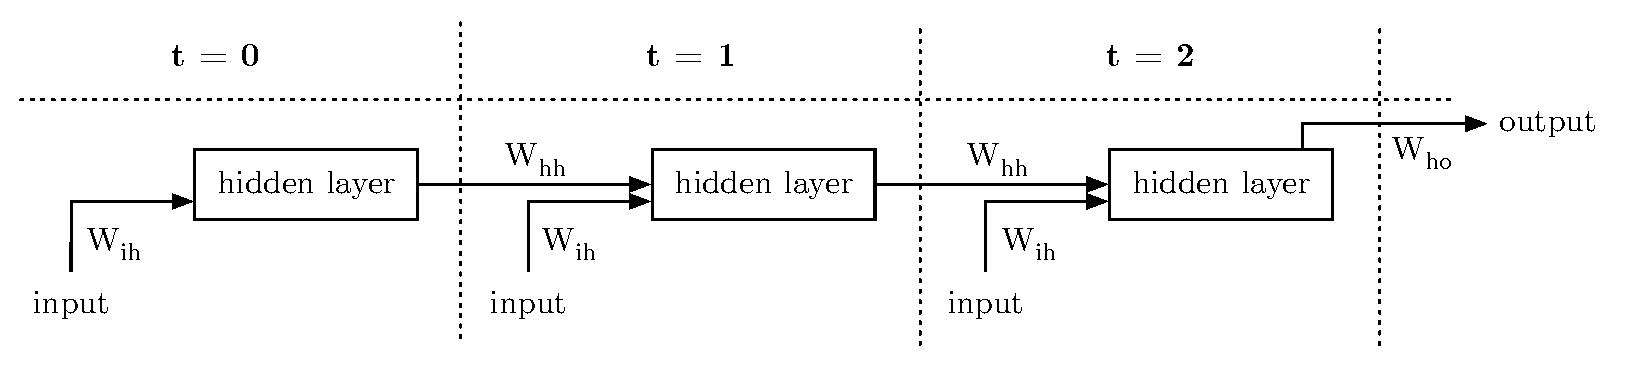
\includegraphics[width=0.8\linewidth]{fig/bptt.eps}
	\caption{Backpropagation through time}
	\label{fig:bptt}
\end{figure}

\subsection{Long Short-Term Memory (LSTM)}
One major issue encountered when using recurrent neural networks is that they
are famous for being unstable. Very often, at some point, training will diverge
(meaning that some gradients will either explode or vanish)
and will never reach a satisfying optimum. Several solutions have been presented
to counter this unstability such as Long Short-Term Memory (LSTM)
cells \cite{lstm}, which we will explain and use in this work, or Gated
Recurrent Units (GRUs) \cite{grus}. \\

\begin{figure}
	\centering
	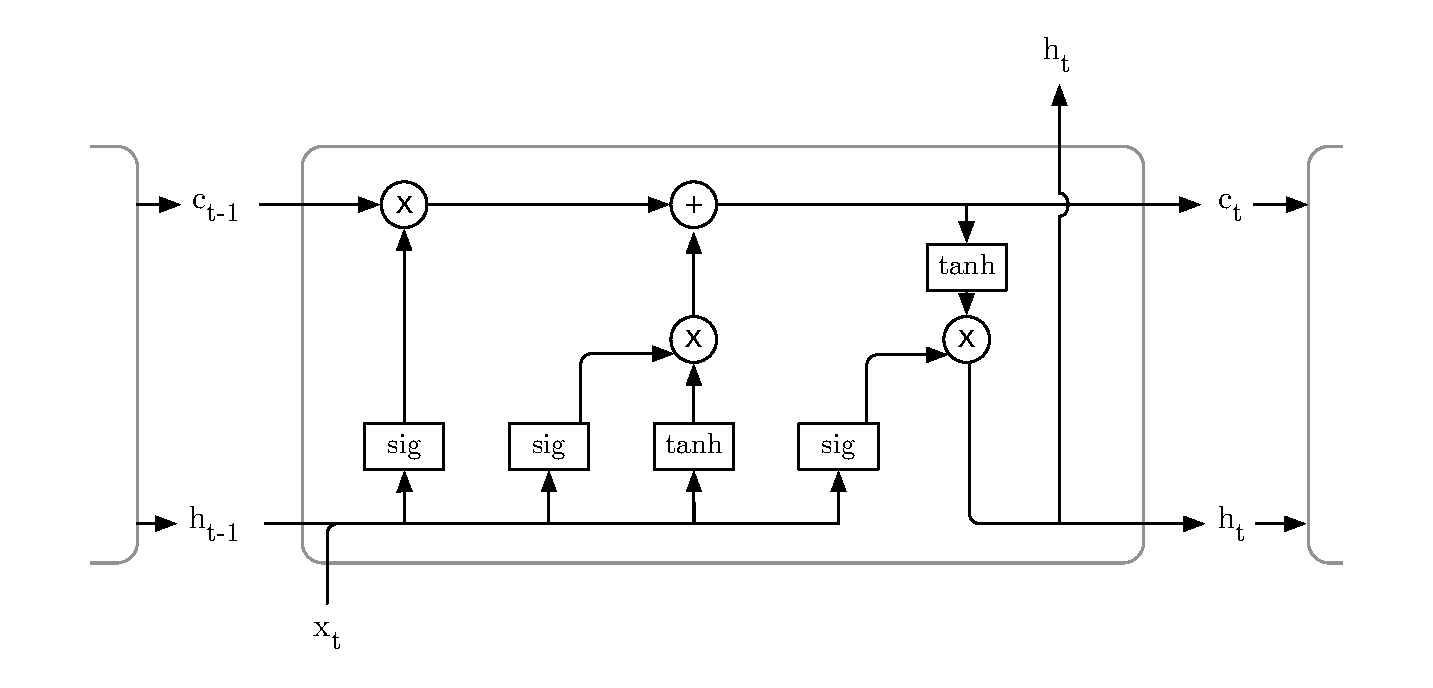
\includegraphics[width=0.8\linewidth]{fig/lstm.eps}
	\caption{The internals of a LSTM cell. Circles represent element-wise
	operations (arrows carry vectors). \framebox{sig} and 
	\framebox{tanh} are layers. $c_t$ is the memory cell.}
	\label{fig:lstm}
\end{figure}

Instead of carrying to the next timestep only the hidden state (which is also
the output of the cell), LSTMs also carry what is called the
\textit{memory cell} $c_t$ which isn't used as output. This memory cell is 
able to handle longer term memory management by using \textit{gates}, which
are rather simple mutliplicative connections, to 
access and modify it. The idea of using gates is to allow the network
to learn to explicitly control its memory by erasing, adding or updating the
information that is in its memory cell.

All gates receive a concatenation of the previous hidden
state $h_{t-1}$ and the new input vector $x_t$. They feed this input through a
sigmoid layer (\framebox{sig})to an element-wise multiplication. There are 
three in total, as they can be seen from left to right on Figure~\ref{fig:lstm}:
\begin{enumerate}
	\item the \textit{forget gate} is the first one. It will multiply each
		value in the memory cell by a value in $[0, 1]$, keeping only
		the values it considers useful.
	\item the \textit{update gate} is the second one and it chooses which
		ones of the outputs of the first \framebox{tanh} layer will
		make their way to the memory cell.
	\item the \textit{output gate} is the last one and decides what parts
		of the memory cell make it to the output.
\end{enumerate}
A deeper analysis of LSTMs and an insight into their behaviour has been
provided by Karpathy et al. \cite{lstm-analysis}
\todo{maybe more?}

\todo{universal function approximators}
\todo{conclusion}


